\chapter{Черторыя}

Она – одна из главных героинь в этой части. Надо познакомиться с Черторыей ближе, иначе ничего нельзя будет понять потом, ни про речку Радунку, ни про городища.

Однако я изменю своему правилу и сделаю несколько важнейших утверждений, не подводя к этому источниками. Доводы изложу позже. Мне нужно быстро, не отвлекаясь, начертать вехи развития Черторыи.

Но прежде кратко изложу популярные знания на 21 век.

Привыкли считать, что левый берег Киева это берег Днепра, а ведь на деле это берег Десёнки и Черторыи, Чертороя. 

На многих картах и в быту Десенка с Черторыей не различаются, ими называют одно и то же русло, что начинается из Десны и на тринадцать километров вдоль левобережья тянется к югу параллельно Днепру, отделенное от него большими островами – Муромцем, да Трухановым с Долобским.

Дачники Русановских садов называют свою речку Десёнкой. На трехверстовой карте Шуберта 1863 года издания, б\'ольшая часть 13-километрового русла подписано «Черторыей», однако до широты троещинской улицы Марины Цветаевой его верховье обозначено как «Старая Десна», что подразумевает – там протекала Десна издревле. На одном плане 1896 года Десной подписано русло Черторыи от Десны до Труханова острова.

На плане Шуберта, 13-километровое русло смыкается с Днепром в двух местах. Северное – пролив Пробитец, между нынешними мостами железнодорожным Петровским и Московским. Теперь там суша – перешеек от Труханова острова к острову Муромцу, выезд с Труханова к Московскому мосту. И южное впадение у моста Метро, через пролив между островами Труханов и Гидропарк.

На некоторых картах Десенка – русло от Десны до бывшего Пробитца, а южнее идет уже Черторыя.

Как же правильно называть эту реку – Черторыя или Десенка, либо это два разных водоема, что соединились?

Вопрос поставлен ошибочно. Ответ будет дан другой, очень неудобный.

Современная Черторыя – русло, поглотившее части других, давних русел. На протяжении веков оно своеобразно развивалось, ползя на север и юг и влияя на смежные водоемы, пока на севере не достигло Десны, а на юге Гидропарка. Рассмотрим, двигаясь по времени от прошлого к настоящему, изменения Черторыи.

\textbf{Итак, утверждение первое} – Черторыя поначалу, как она возникает в летописных упоминаниях, это водоем около Труханова острова, однако не севернее.

Слово «черторыя» или «черторой», по словарю Даля, означает «овраг, рытвина от воды». На карте Украины раскидано много Черторый. Даль знал также пролив «Пробитец, под Киевом, соединяет Черторою с Днепром».

В летописях, по времени сообщения, Черторыя впервые появляется в Воскресенском и Никановском списках, а это списки новые, 16 века. Сведения относятся ко времени Гюрги – Юрия Долгорукого.

Вот что сообщает Никановская летопись, за 6658 год (1150):

\begin{quotation}
а князь Юрий Долгорукий Владимерич Маномашь в то же время приде к Киеву з Давыдовичи и Олговичи, и ста у Черторьи\footnote{Воскресенская летопись: «ста у Черторыи».}, и посла за Изяславом Мстиславичем князя Святослава Всеволодича и сына своего князя Бориса, и гнаша по нем до Чертова леса, и не достигше воротишася вспять 
\end{quotation}

Старинная Ипатьевская летопись излагает то же иначе – делаю сокращения, выпуская всё не касающееся вопроса:

\begin{quotation}
И в то веремя приде Гюрги с сынми своми, и Володимир, Изяслав Давыдовича, и Олгович Святослав, и сыновец его Святослав Всеволодич, над берег противу Киеву.

Кияне же мнози поехаша в насадех к Гюргеви, а друзии почаша в насадех дружину его перевозити на сю сторону в Подолье.

Вячеслав же с Изяславом рекоста видивша то: «на нею веремя ныне есть». [...]

В втрий же день приде Володимер Галичьской к Олгове могыле, тако же и Дюрги приеха к нему [...] и ту ся целоваша не съседаюче с коний, у Сетомля на болоньи; сдумавше послаша по Изяславе Святослава Всеволодича, Бориса Дюргивича. и гониша но них до Чертова леса, и не постигше их, взвратишася.
\end{quotation}

Что же, здесь нет Черторыи, сказано просто «над берег противу Киеву». И – мы разберем это далее – в описании попыток Гюрги захватить Киев, Ипатьевская летопись не упоминает Черторыю среди прочих урочищ.

Я полагаю, что Никоновский и Воскресенский список напрасно уточняют «ста у Черторыи» – ее тогда, для времени описываемых событий, просто не существовало. А в 16 веке – несомненно, уже была. Да и гораздо раньше.

Та же Ипатьевская летопись за 6688 (1180):

\begin{quotation}
Святослав въеха с братома  Киев. Половци же испросиша у Святослава Игоря, ать ляжет с ними по Долобьску, Святослав же отпусти.

[...]

Половци же бегаючи перед Русью потопоша мнозе в Черторыи, а инех изимаша, а другыя иссекоша.

[...]

Игорь же виде Половце побежены, и тако с Концаком вскочивша в лодью, бежа на Городец к Чернигову.\end{quotation}

Половцы с Игорем расположились по Долобську (из летописи нельзя понять, местность это или водоем), затем воины, состоящие из Руси, начали их громить и Половцы тонули в Черторыи. Игорь, однако, где-то там вскочил в лодью и умотал в Городец к Чернигову (это другой, не киевский Городец). Значит, тогда был некий водный путь от Долобська к Десне.

По этим летописным сведениям мы можем только и понять про близость Долобська и Черторыи, да что Черторыя была водоемом достаточным для утопления Половцев. %Возможно, еще в летописные времена Черторыей стали называть рукав Днепра около Труханова острова, но прямых указаний на это в источниках нет.

\textbf{Утверждение второе} – на 16 век, Черторыя это водоем южнее Воскресенки, всё еще на уровне Труханова острова.

\textbf{Третье} – на 17 век, в Черторыю севернее Труханова острова и Московского моста (где нынешний остров Муромец) пробивается рукав Днепра. Таким образом протяженность Черторыи увеличивается на север. Однако, Черторыя еще не соединена своим устьем с Десной. Покамест устьем Черторыи можно считать этот рукав Днепра.

Дальнейшие века.

1. В Черторыю с севера пробивается Десна, а рукав Днепра (по нынешнему острову Муромцу) пересыхает, «отпадает». Устьем Черторыи становится Десна.

2. Днепр снова пробивается в Черторыю уже на широтах Московского и Петровского мостов – так возникает пролив Пробитец, а ниже его русло Черторыи раздувается.

Таковы важнейшие вехи развития Черторыи.

Название же Десенка рождается, кажется, в 19 веке, для обозначения русла Черторыи от широты Пробитца до устья у Десны. Термин «Десенка» широко используется в гидрологических текстах стыка 19-20 веков, где Десенкой считают рукав Десны, а Черторыей – рукав Днепра, и Десенка впадает в Черторыю. Таковы были представления, например, известного инженера, гидролога Николая Максимовича. В этой книге я применяю название Черторыя ко всему современному руслу от Десны до Гидропарка, и к руслу меньшей протяженности в давнее время, о чем буду говорить особо.

Максим Берлинский в 1820 году написал\cite{berl01} про Черторыю и Пробитец, тогдашнее их значение:

\begin{quotation}
Черторыя.

Речный судопроходный рукав, отделяющийся от Десны близ устья ея, протекающий по луговой стороне против Киева, и наконец сливающийся с Днепром против самаго Николаевского монастыря\footnote{То есть на уровне Дворца Пионеров и Аскольдовки.}, из стари и теперь называется Черторыею.

На средине своего течения соединяется она также с Днепром  посредством течения пролива, называемого Пробитцем. Сей Пробитец учинился с 1777 года от напору реки, когда предприняли было каменною гатью на Днепре отворотить его стремление от Киева-Подола в Черторыю.

Теперь сим Пробитцем проходят суда в глубокую Черторыю, избегая многих непостоянных отмелей, бывающих у Киева на Днепре.
\end{quotation}

Иными словами, вместо плавания от Подола сразу вниз по Днепру вдоль правого берега, поднимались по течению чуть выше, зачем через Пробитец шли в Черторыю и ею спускались в Днепр же на широту немногим севернее нынешнего моста Метро. А прежде того, в 1777 пытались отвести воды Днепра в Черторыю при помощи каменной гати, дабы Днепр не заливал в половодье Подол.

И. Ф. Тимковский в сочинении «Мое определение в службу. Сказание в 3-х частях. Писано в 1850 г.» сообщал:

\begin{quotation}
и как Днепр, отбиваемый устьем Десны, всякий год весною на Подоле к Оболонью разом обширно заливал и вырывал берег, и мы видели тогда плывущими на нем избы, сараи, обломки: то в 1788 году, для отвода его, разрывали у левого берега рукав, Черторый, поденной платою вольноприходящим от голову до 3 коп. Теперь слышно, что полагают запереть Черторый, для обмелевшего Днепра.
\end{quotation}

В 1840-50 годах Черторыю в районе между современными Московским и Петровским мостами, наоборот, отделили от Днепра запрудой, чтобы из Днепра вода не уходила налево. А запруда из Десны в Десенку впервые была построена в 1884-м, после чего в Десенку стало уходить меньше воды.

%Гидролог, инженер Максимович писал, что в конце 18 века в истоке Черторыи (у Десны) сделали запруду, затопив там байдаки с камнями, чтобы вода шла дальше по Десне через ее устье и питала обмелевший Днепр. Теперь в истоке Четорыи – тоже дамба и первый водозабор Деснянской водопроводной станции.

\begin{center}
\includegraphics[width=\linewidth]{chast-gorodki/cherto/s_mur_CRW_3927.jpg}

\textit{Заводь Черторыи на острове Муромце. 2014 год.}
\end{center}
 
Современная Черторыя принимает в себя все левобережные воды на протяжении от Десны до моста Патона. Течение в Черторые быстрее, нежели в Днепре, глубина порядочная – на разных участках фарватера от 15 до 9 метров, конечно есть и мельче. При сопоставлении с Днепром можно сказать, что Черторыя на одних с ним широтах течения обычно чуть глубже, однако немного \'уже. Например, в районе Московского моста, с южной его стороны, глубина фарватера Черторыи равна 8 метрам, а Днепра – только 6 метров. У Труханова острова напротив Подола, фарватер Днепра – 7-9 метров, а по другую сторону Труханова, Черторыя дает 9-14 метров.

Я даже не говорю о чудовищных заливах к югу и северу от проспекта генерала Ватутина – дно их это ямы до 20 метров глубиной, образовавшиеся от добычи песка. В середине 20 века здесь был большой остров в Черторые, отрезанный с востока от материка озером Неводным, давним остатком того русла Черторыи, когда в него не вливался еще Днепр около Петровского моста. От острова сохранился участок между Московским мостом и перекрестком улицы Бальзака с проспекта Ватутина. Нижний залив известен ныне как «залив Десенка».

А на дикой местности непосредственно к северо-запа\-ду от перекрестка, был и остается водоем с рыжей водой\footnote{Исток: 50°30'17"N  30°34'38"E, устье: 50°30'2"N 30°34'8"E.}, про него я поведаю позже, ибо разговор будет долгим.

В 19 и по середину 20 века, от Десны на юг примерно до Петровского железнодорожного моста, русло Десенки было, в отличие от теперешнего, довольно узким, ну – чуть шире проспекта Генерала Ватутина. А вот дальше вниз – как придется, местами почти с Днепр. Почему так? Да потому, что южнее моста в Черторыю грубо вторгся Днепр, и русло первой одно время несло в себе воды и Днепра, сомкнувшись с ним Пробитцем в точке между островами Муромцем и Трухановым.

За столетия существования и развития, Черторыя отобрала поглотила много водоемов, отрезала от материка несколько островов и со временем дошла до нынешнего моста Патона. Когда там находилось устье Черторыи, Гидропарк был островом. А до конца 19 века превратился в полуостров, продырявленный озерами и остатками прежнего русла Черторыи. Её – на уровне Николаевского моста и позже выстроенного почти на его месте моста Метро – Днепровской дамбой свернули на запад к Днепру. 

Через Днепр, от острова до Киева, в 1850-х по проекту Чарлза Виньоля построили Николаевский цепной мост. Основу его составили пять кирпичных опор, или «быков», пролеты между ними поддерживались цепями, закрепленными в арках. Цепи были из двухсоткилограммовых звеньев, каждое длиной в 3,6 метра. На правом берегу у моста соорудили пятикупольную часовню святого Николая, и с Печерска подвели Николаевский спуск, именем связанный с издавна стоявшим выше, на горе, Никольским Пустынным монастырем и церковью святого Николая на Аскольдовой могиле.

\begin{center}
\includegraphics[width=\linewidth]{chast-gorodki/cherto/\myimgprefix nikmost01.jpg}

\textit{Николаевский цепной мост и Предмостная слободка.}
\end{center}

Красавец-мост, архитектурное чудо, ставшее одной из знаковых частей города, прослужил людям около семидесяти лет. А 10 июня 1920 года из Киева драпали польские войска, чей командующий, Эдвард Рыдз-Смиглы, приказал уничтожить мост. Для этого понадобилось немного – по заряду взрывчатки на каждую несущую цепь. Пролеты упали в воду. Там их вместе с цепями взорвали год спустя уже наши, чтобы суда могли плавать.

На следующей фотографии, 1920 года, хорошо видно эти ослабленные цепи, и юго-восточную часть Предмостной слободки с церковью Иоанна Рыльского, справа. А дальше, по Броварскому шоссе выглядывает Николаевская церковь\footnote{Снесена в 1961 году при проложении линии метро. Краеведы любят рассказывать, что в ней венчались Гумилев с Ахматовой.} – это уже через Русановский пролив (теперь он – от моста Метро и до Патона, вдоль Русановки), в Никольской слободке! Церковь Иоанна Рыльского была возведена в 1909 году на средства Варвары Бобриковой, 20500 рублей, в память о погибшем на войне муже Иване. Закрыта в 1935-м с передачей здания под общежитие рабочим, что строили школу. Сгорела в 1943 году вместе со Слободкой.

\vspace*{\fill}
\begin{center}
\includegraphics[width=\linewidth]{chast-gorodki/cherto/1920-cep.jpg}
\end{center}
\vspace*{\fill}
\newpage

Руки, а главное – голова – до восстановления моста через Днепр дошли только в 1925-м. Евгений Патон, надстроив опоры старого моста, поставил сверху новый, на него очень похож современный Пешеходный. Мосту присвоили имя Евгении Бош, которая застрелилась в том же году. Бош – профессиональный революционный деятель из тех, кто в мирное время не расстается с маузером. Мать двоих детей, она не научилась ценить ни чужие жизни, ни свою.

19 сентября 1941 года наши войска при отступлении уничтожили за собой мосты – взорвали железнодорожный мост имени Петровского, мост Евгении Бош, южный Дарницкий, да спалили, облив смолой и бензином, деревянный Наводницкий мост. Живучие опоры Николаевского моста и после войны торчали из воды, пока рядом не построили мост Метро.

Прежние опоры видны в старых фильмах, например в комедии «Она вас любит» с Вицыным, где он играет роль ветеринара зоопарка. В 1960-х опоры взорвали, уцелевшие остатки трех ныне затоплены, ведь после запуска Киевской и Каневской ГЭС уровень воды в Днепре у Киева поднялся. Но когда река сильно мелеет, опоры заметны, как было весной 2010 года.

После сооружения Николаевского моста, на будущем Гидропарке стали селиться рабочие с правого берега и возникла Предмостная, или Ближняя Никольская слободка, она же Печерская.

В Гидропарке Николаевский мост не был первым. Раньше на его месте уже существовала переправа, наводили плавучий Спасский мост\footnote{По имени очень крутого Спасского спуска, а тот назван от близости к церкви Спаса на Берестове, что стоит выше на горе. О перевозе через Днепр по сему месту сказано еще в книге «Тератургиме» лаврского ученого монаха Афанасия Кальнофойского, в 1638 году.}, а другой был южнее около удолья Наводничей (между ними и Лаврой), и на левом берегу подходил к старинной дороге в Дарницу, у Резановского трактира с постоялым двором. По крайней мере с середины 18 века, за сим мостом, по левому берегу на север шла дорога к Никольской слободке, сворачивая затем на восток к Москве.

Давний путь, известный ныне под именем Броварского шоссе, прежде раздваивался. Одна ветвь соединялась с ним от Наводницкой переправы, другая – от Спасского моста. Последняя существовала уже в 1830-х. Сразу за Спасским мостом начиналась дорога, по деревянному мосту переваливала через Русановский пролив – нижнюю часть Черторыи, и материком направлялась к Никольской слободке (Левобережка) и дальше.

В начале 20 века деревянный Русановский мост заменили металлическим двухпролетным, по проекту Николая Аполлоновича Белелюбского, а также инженера Григория Кривошеина и архитектора Владимира Апышкова.

По нынешней линии метро в Гидропарке и Русановскому мосту была устроена Днепровская дамба. Вот Гидропарк конца 19 века в «разрезе», с севера на юг (из «Пояснительной записки к проекту окончания выправительных работ на р. Днепре у г. Киева», Николая Максимовича, изданной в 1896 году). Показаны, кроме прочего, два засыпанных моста.

\begin{center}
\includegraphics[width=\linewidth]{chast-gorodki/cherto/1896-profil.jpg}
\end{center}

В 1912 году в Дарницу (там где сейчас Дарницкий вокзал) через оба моста, Николаевский и Русановский, проложили линию мото-трамвая от Почтовой площади до железнодорожной станции «Дарница». Билет туда из Киева стоил 20 копеек\footnote{В больших городах, средняя зарплата рабочего составляла тогда около 22 рублей. Чернорабочий получал 120 копеек в день, токарь – 250. Кочан капусты стоил около 18 копеек, десяток яиц – 30 копеек, фунт ржаного хлеба – 3 копейки.}, трамвай ходил раз в 20 минут.

\begin{center}
\includegraphics[width=\linewidth]{chast-gorodki/cherto/s_rusmost.jpg}

\textit{Русановский мост. Дореволюционная открытка.}
\end{center}

Депо линии находилось в Никольской слободке. Спустя год открыли вторую линию аж до Броваров\footnote{Эти трамвайные маршруты уже в 1930-х получили номера с 14 по 16, а после Великой Отечественной их не возобновили.}!

Население острова росло. На 1917 год в Предмостной слободке обитало 7200 человек. В северной части поселка были улицы: Днепровская дамба, Баглеевская, Лосенская, Ольгинская, Венецианская, Адамовская, Украинская, Пароходная, Судовая, Мариинская, Тенистая, Монетная. В южной: Русанов вал, Тупая, Южная, Женевская, Успенская, Анненская, Московская, Киевская, Шереметьевская, Трояновская, Струмиловская, Торговая, Николаевская, Днепровская набережная, Заводская, Троицкая, Аскольдовая, Вербиловская, Луговая, Дарницкая, Луговое шоссе, переулки Музен, Кривой, Днепровский. Дома строили на сваях. В половодье жители плавали по улицам в лодках.

Некоторые дворы соседствовали с озерами. Церковь стояла к югу от моста, близко к Днепру – теперь там, у обочины кольца развязки, памятный черного камня крест, заметный из вагона метро, если глядеть в сторону моста Патона. Чуть дальше от берега, вглубь острова, где ныне теннисные корты, шумел базар, а за ним пряталось озерцо. По другую сторону от него, через Броварское шоссе, были пруд, парк с рестораном «Венеция» (он же Петровский, вход от 40 до 50 копеек) и частная дача. Со слободки вело три пути. Западный, на правый берег – через Николаевский мост. Восточный – на Никольскую слободку по Русановскому мосту, через одноименный пролив, естественное продолжение Черторыи. Юго-восточный – по мостику над меньшей протокой Черторыи и дальше в Дарницу.

К концу 19 века Предмостная слободка вновь оказалась на острове, ибо с юго-востока ее отр\'езал от материка Русановский пролив. Он разделялся надвое. Широкий рукав сохранился целиком – ныне он течет вдоль берега Русановской набережной.

А от меньшего рукава, пересекавшего слободку, остались залив в восточной стороне Гидропарка (видно с Русановского моста, за лодочной станцией) и озеро посреди острова. Именно через этот пролив был мостик к дороге в Дарницу, когда большее, второе русло пролива существовало как цепь озер и по суше между ними шла дорога.

Так восстановился уже некогда существовавший отрезок низовий русла Черторыи, да снова образовался остров, омываемый Днепром и Черторыей – будущий Гидропарк. Русановский пролив от моста Метро (левобережного участка) доходит до моста Патона и воды его смешиваются с днепровскими.

В 1877 году цепь озер превратилась в полноценный, большой пролив. Гидрограф Максимович пояснил причину:

\begin{quotation}
Весною 1877 года, при весьма высоком подъеме весенних вод, деревянные мосты в Днепровской дамбе были снесены водою, а в отверстие наибольшего из них, так называемого Русановского, образовалось новое речное русло, по которому направилось речное течение со значительной силой. 
\end{quotation}

\newpage
\vspace*{\fill}
\begin{center}
\includegraphics[width=\linewidth]{chast-gorodki/cherto/\myimgprefix pslob02.jpg}

\textit{Предмостная слободка дореволюционная.}
\end{center}


\begin{center}
\includegraphics[width=\linewidth]{chast-gorodki/cherto/predm-s-prevber.jpg}
\textit{Вид на слободку с правого берега.}
\end{center}

\vspace*{\fill}
\newpage
\vspace*{\fill}
\begin{center}
\includegraphics[width=\linewidth]{chast-gorodki/cherto/\myimgprefix pslob03.jpg}

\textit{Предмостная слободка дореволюционная.}
\end{center}


\begin{center}
\includegraphics[width=\linewidth]{chast-gorodki/cherto/\myimgprefix 3265.jpg}

\textit{Вид с нее на правый берег.}
\end{center}
\vspace*{\fill}
\newpage
\vspace*{\fill}
\begin{center}
\includegraphics[width=\linewidth]{chast-gorodki/cherto/\myimgprefix 546547567.jpg}

\textit{Вид на нее с правого берега.}
\end{center}

\begin{center}
\includegraphics[width=\linewidth]{chast-gorodki/cherto/predmost.jpg}

\textit{Половодье в слободке.}
\end{center}
\vspace*{\fill}
\newpage

На Русановской набережной есть Плавни. Это поросший лозами мыс, где вовсю дымят шашлыками, пьют пиво, громко включают музыку и отчаянно мусорят – словом, весь тот набор почестей, которые способен оказать природе современный киевлянин. Там же дикий пляж, доходящий до бетонного северного берега Русановского канала. 

Я помню Плавни восьмидесятых годов, тихие и чистые, запах ивняка, какие-то старые деревянные лодки в мелких заводях. Весной, местные ходили сюда ломать на продажу «котики», пушистые соцветия вербы.

Плавни лежат напротив места, где Русановский пролив раздваивался. В 1950-х мыс Плавней еще более выдвигался на запад, почти перешейком между материком и островом, прорезанный двумя руслами. И если бы не очередное вмешательство человека, то протоки, при тогдашней системе запруд, снова бы обмелели и Гидропарк превратился в полуостров.

В восьмидесятые, от Русановской набережной на восточный берег южной части Гидропарка ходил катер. Узкий пляж, белый песок, лозы. 

С другой стороны острова, напротив парка Примакова, тоже был пляж, и причал с катером. Тот пляж считался нами, жителями Зверинца, главным. Я тогда не воспринимал его как Гидропарк, хотя так называли весь остров.

Гидропарк для меня был связан с аттракционами, куда мы добирались на метро. Еще не воняло шашлыками, люди мирно гуляли по бетонным плитам дорожек и пили воду из фонтанчиков.

Дорожки приводили нас с мамой к цепным каруселям и качелям-лодочкам. К сталкивающимся, с резиновыми буферами, электрическим машинкам, что сыпали искрами и пахли горелым. К павильону игровых автоматов. Как я любил морской бой! Суешь лицо в пахнущую резиновую маску перископа. Видишь в зеленом свете поле боя, а руки лежат на таком руле с гашеткой. Под большим пальцем кнопка выпуска торпеды. Пууу! И враг повержен.

Больше всего мне нравились американские горки, но катался на них я всего дважды. Страшно! Вышка, с нее два дюжих мужика пускают по деревянному желобу вагонетки. Желоб идет буграми вверх-вниз и потом ныряет в бетонный тоннель, что едва не сносит тебе голову. Я не знал, что в Гидропарке были вещи страшнее.

Незадолго до освобождения Киева советскими войсками, 26 сентября 1943 года немцы стали жечь Предмостную слободку, купно с Никольской и поселком на Трухановом острове. Через обе слободки наши прорывались с боем. 28 сентября в час дня подразделения 56-й гвардейской танковой бригады\footnote{Из состава 3-й танковой армии генерала  Рыбалко.} вошли в Никольскую слободку, но были остановлены тремя противотанковыми рвами и минным полем. Обезвредив 250 мин, подразделения пошли дальше на Предмостную и к пятнадцати часам освободили ее от немцев.

В боях за окрестности Дарницы участвовали также части 163-й и 136-й дивизии 50-го стрелкового корпуса 38-й армии Воронежского фронта\footnote{50-й стрелковый корпус генерала Мартиросяна, 136-я стрелковая дивизия полковника Пузикова, 163-я стрелковая   дивизия полковника Ф. В. Карлова.}. В тот день, выбивая врага из-под Броваров, чтобы подойти к Дарнице, в бою участвовала Мария (Маруся) Лагунова, двадцатидвухлетняя механик-водитель танка Т-34. Родом с Урала\footnote{Родилась в деревня Оконечниково Катайского района, в четыре года осталась без матери, окончила пять классов школы, перебралась к сестре в Свердловск, работала нянькой, в 16 лет устроилась на «Уралобувь» электриком, в свободное время училась водить заводской грузовик.}, доброволец. Фрицы подбили ее танк из пушки. Маруся лишилась обеих ног, однако научилась ходить на протезах без помощи костылей и вернулась в армию\footnote{Долгие годы солдаты танковой части, где служила Лагунова, считали, что она умерла под Броварами, ибо командованию доложили, будто Маруся скончалась от ран по пути в госпиталь. Уже после войны однополчане узнали из прессы, что Лагунова жива, и связались с ней.}. Демобилизовалась уже после войны.

Прожила достойную жизнь, умерла в 1995-м, в Броварах. В былое время там каждый знал, где живет Лагунова – на улице Энгельса. Ныне память хранит музей школы №41, да улица, названная в честь Маруси. 
\vspace*{\fill}
\begin{center}
\includegraphics[width=\linewidth]{chast-gorodki/cherto/predmost-j.jpg}

\textit{Наши залегли в Предмостной слободке, напротив Лавры.}
\end{center}
\vspace*{\fill}
\newpage
\vspace*{\fill}
\begin{center}
\includegraphics[width=\linewidth]{chast-gorodki/cherto/predmpojar-j.jpg}

\textit{Гитлеровец наблюдает за гибелью Предмостной слободки.}
\end{center}
\vspace*{\fill}
На восток от Предмостной, через Русановский мост над Черторыей (или, если угодно, начало Русановского пролива), лежала Никольская слободка («дальняя Никольская слободка», основная), теперь это окрестности станции метро «Левобережная». Обе слободки в быту часто совмещались, назывались просто Слободкой, или же именование Никольской распространялось и на Предмостную. Никольская «континентальная» прожила долгую жизнь, постепенно застраиваясь новыми зданиями. Еще в 2005 году на месте нынешнего супермаркета «Новус», почти против станции метро были остатки частного сектора. На видео это можно посмотреть в самом конце \href{http://www.archive.org/download/Kaleidoscope/kld_mpeg4.avi}{фильма «Калейдоскоп»}, снятого любительской студией «Дрымба». За строительным забором, во фруктовом саду запорошило снегом хату с проломленными стенами из дранки, деревянный сарай, будку туалета. И сад тот вырубили.

\newpage
\vspace*{\fill}
\begin{center}
\includegraphics[width=\linewidth]{chast-gorodki/cherto/\myimgprefix nslob.jpg}

\textit{Никольская слободка на дореволюционной открытке.}
\end{center}

\begin{center}
\includegraphics[width=\linewidth]{chast-gorodki/cherto/8865d6c145cea5226cd9f1a60f599465.jpg}

\textit{1960-е, вид на метро с юга.}
\end{center}
\vspace*{\fill}
\newpage
\vspace*{\fill}
\begin{center}
\includegraphics[width=\linewidth]{chast-gorodki/cherto/s_niksl_DSC_0044.JPG}
\end{center}

\begin{center}
\includegraphics[width=\linewidth]{chast-gorodki/cherto/s_niksl_DSC_0048.JPG}
\end{center}

\textit{На снимках 2013 года – северная часть слободки.}
\vspace*{\fill}
\newpage

К Никольской слободке, северной ее части, относится и частный сектор, примыкающий с юга к Русановским садам, там где улицы Сагайдака, Чаадаева, Силикатная, Комбинатная (от Дарницкого комбината строительных материалов и конструкций, к нему подходила Комбинатная и ветка железной дороги). На 2016 году большая часть территории завода застраивается жильем.

В восточной части слободки, точно перед нынешней больницей №2 на основной районной улице – Луначарского, было слободское кладбище. Теперь там сквер.

Еще одна потеря слободки – озеро Свят\'ище, Святищево или Свят\'ыще, занимавшее место юго-восточной части Русановского канала от моста возле улицы Раисы Окипной и до моста около улицы Ованеса Туманяна. Иначе говоря, часть канала на отрезке вдоль улицы Флоренции раньше был озером. Впервые я встретил его на моем любимом плане Даниила де Боскета 1750 года:

\begin{center}
\includegraphics[width=\linewidth]{chast-gorodki/cherto/s_svyat-1750.jpg}
\end{center}

Здесь видно – к югу (слева) от Никольской слободки, но севернее «дороги в Бровары» – Лысую гору и озеро «Светищево» с мостом через оное. 

Лысую гору мы обсудим позже. Сейчас про озеро. Некоторые краеведы полагают, что оно сгинуло еще в начале 20 века, однако на аэрофотоснимке 1943 года длинное Святище – вот оно, живо-здорово, в середине картинки:

\begin{center}
\includegraphics[width=\linewidth]{chast-gorodki/cherto/svyat-1943.jpg}
\end{center}

В то время параллельно северному берегу озера проходила улица Лозовая, да к самому озеру шли два проулочка.

Именно на берегу бывшего Святища, в конце улицы Туманяна стоит высотный дом номер 8, последний адрес актера и режиссера Леонида Быкова. Вообще Русановский канал почти точно вписался в изогнутую цепь тамошних водоемов, сохранившихся на 20 век – Святище, болото, Тельбин.

Сейчас на картах именем «Святище» обозначено другое озеро, на Осокорках.

А как долго я весной 2013 года искал настоящее Святище, не зная тогда об аэрофотоснимке! В первый день поиска я бродил между станцией метро «Левобережной» и Русановским каналом, одетый по случаю отцовского дня рождения в солидный пиджак. Много лет, после детства, я не носил пиджаки, а этот подкупил меня обилием карманов и подкладкой, не вызывавшей судорог души. Я вглядывался в каждую низину между домами. Потом поехал туда же на велике, и во глубине дворов нашел большую ложбину, с детской и баскетбольной площадками. Где и заподозрил Святище, пока не понял по аэрофотоснимку и новым для меня картам, что озеро поглощено каналом.

\begin{center}
\includegraphics[width=\linewidth]{chast-gorodki/cherto/s_svyat-IMG_20140527_134118.jpg}
\textit{Тут было озеро Святище. Май 2014 года.}
\end{center}

В XXIX томе журнала «Киевская старина», за 1890 год, помещена статья археолога Николая Беляшевского\footnote{Любопытно, что Беляшевский вел раскопки и близ другой Лысой горы, на Кирилловских высотах, где исследовал знаменитый Курган-могикан.} «Первобытный человек на берегах р. Днепра», где он рассказывает о находках возле Святища. Ценность этого сообщения еще и в описании места, каким оно было в конце 19 века:

\begin{quotation}
Бугры у с. Никольской Слободки. С. Никольская Слободка находится в том месте, где кончаются сооружения Цепного моста и начинается Черниговское\footnote{Ныне Броварское.} шоссе. 

К югу от села, сейчас же за ним, лежит небольшое озеро Свят\'ыще. Песчаные открытые бугры составляют северо-восточный берег этого озера, они простираются затем с одной стороны к лесу, с другой же подходят к постройкам идущим в этом месте по обеим сторонам шоссе.

По другую сторону шоссе пески также обнаруживаются и заканчиваются большим бугром в северном конце села у сельского кладбища. Ближе к лесу бугры покрыты тонким слоем дерна и отчасти окрайной леса.

Обнажения культурного слоя заметны главным образом по берегу озера и на такой высоте, что вода в весенние разливы туда не добирается; в этом можно было убедиться во время сильного разлива весной 1888 г.; местность же между этим берегом озера и противоположным правым берегом Днепра, представляет весной сплошную водную поверхность.

Находки сосредоточивались в двух местах: при начале озера, там, где кончалось село, и даже крайние хаты его уже расположены на обнаженном культурном слое, и затем – почти в конце озера, – здесь культурного слоя почти не было заметно, но зато найдено несколько сосудов.

Случай дал возможность сделать и геологические наблюдения: летом 1889 г. из берега озера брали песок для земляных работ на реке; в образовавшейся выемке было видно, что однородный светло-желтый песок залегает на несколько сажней вглубь.

Внешний вид местность по берегу озера имела следующий: песок окрашен в пепельно-се\-рый цвет, толщина темного слоя различна – иногда достигает 1/4 аршина\footnote{Около 18 сантиметров.} и более, иногда же является как бы тонким налетом. На поверхности разбросаны, а также торчат из песка куски от сосудов с орнаментом и без него, лежат также черепки и кучами, они, по-видимому, принадлежали целым сосудам, распавшимся от действия атмосферы; между черепками много измельченных выветрившихся костей, встречающихся также кучами, и масса осколков кремня и других камней, между ними попадаются и кремневые орудия.

Местами все эти остатки расположены вокруг кострищ, представляющих не особенно большие кучи углей. Это в начале озера. Дальше по берегу культурного слоя не было замечено, но попадались черепки, а при конце озера вблизи кострищь найдены были, как уже сказано, целые сосуды.

[Далее Беляшевский начинает опись находок, привожу ее далее в пересказе.]
\end{quotation}

Целыми нашли немного орудий, большинство же – поломанные. 80 обоюдоострых ножиков из кремня (наибольший из которых был длиной 5,5 см., а шириной 1) отличались, по словам Беляшевского, миниатюрностью, как и все остальные орудия. 7 кремневых острий длиной до 3 сантиметров. Кремневые наконечники стрел около 20 штук, обнаружены почти вместе, там же где осколки кремня. Полсотни овальных кремневых скребков. Про множество поломанных орудий Кибальчич высказал мысль, что их могли разбивать нарочно при погребальном обряде.

Керамические изделия не знали гончарного круга, лепились руками. Беляшевский пишет:

\begin{quotation}
Глина выделывалась различно: встречались (редко) черепки из грубой глины с большою примесью кварца, затем из глины лучшего качества, но все-таки не обладавшей достаточным сцеплением, наконец были из глины хорошо отмученной, неуступающей современной.

Обжиг также различен; это можно видеть на изломе черепков; большей частью обожжена только наружная сторона, получившая от этого красный цвет.

[...]

был также и полный обжиг, прошедший насквозь черепок. Толщина стенок сосудов от 1 1/2 до 1/2 сантиметра.
\end{quotation}

Сосуды были до 20 сантиметров в поперечнике, а высотой до 30 сантиметров. Узоры в виде точек,  прямых линий и зигзагов сделаны по сырой еще глине палочкой, костью, кремнем, веревочкой. Ушек сосуды не имели, вместо этого проделаны дыры ближе к ободу. Среди глиняных предметов Беляшевскому попалось глиняное прясло и обломок другого.

Кроме того археолог нашел там же, в песке, предметы, отнесенные им к более новому времени – бронзовые куски пряжек, перстней, пуговиц, бубенчик, кольцо, трехгранные стрелы. А также железные «стрелы разных форм и ножички».

По уровню гончарного мастерства и отделки кремневых наконечников, Беляшевский отнес культурный слой к концу каменного века и концу его неолитического периода. Ученый полагал, что отыскал здесь стоянку первобытного человека.

И далее в статье дается замечательное, современное ей описание смежной местности, которое нам пригодится, чтобы знать, как выглядел тогда Левый берег:

\begin{quotation}
К северу от Никольской Слободки, на протяжении почти 5-ти верст вплоть до с. Воскресенского, тянется под лесом ряд бугров различной величины и формы\footnote{Речь идет о длинной возвышенности, слывущей Лысой горой – однако не к югу как отмечено на карте 1750 года, а по другую сторону от Никольской слободки, на север.}, покрытых тонким слоем дерна. В некоторых местах дерн разрушился, песок обнажился и, вследствие действия ветра, образовались небольшие котловины; в них попадаются хотя и в незначительном количестве аналогичные с найденными у Никольской Слободки черепки и кремни, так что бугры эти являются продолжением стоянки Никольской слободки.

У села Воскресенского бугры принимают более правильную куполообразную форму и совсем обнажены; находки и здесь были самые незначительные.

Рядом с селом Воскресенским идет ровная песчаная плоскость, не давшая никаких находок; только в конце, где опять начались бугры, найдено несколько отбивных кремней и большая, хорошо подправленная стрела. 

Эти же бугры тянутся далее вокруг болота, отделяющего село Воскресенское от лежащего выше села Вигуровщины. Там, где болото более всего вдается в берег, обнаружено небольшое место, сплошь покрытое осколками кремня, кусками ножиков\footnote{Почему-то всюду не ножи, а ножики – маленькие.}, целыми ножиками и скребками, тут же [...] лежали осколки розоватого песчаника, из которого хотели приготовить орудия.

Между черепками по орнаменту были одинаковые с найденными у Никольской слободки, но нашлось также и несколько особенных, как например орнамент елкой.

Целых сосудов у села Вигуровщины не было найдено, но нам передавали местные пастухи, что весной они часто находили в песке «якись мыски». Встречались в кучах черепки от распавшихся сосудов.

[...]

Далее села Вигуровщины мы не простирали наших изысканий, но в этом месте бугры, продолжаясь немного выше по направлению к селу Троещине, прекращаются и опять обнаруживаются, насколько мы знаем, уже спустя большое пространство\footnote{Подобная цепь песчаных холмов, более короткая – урочище Сухие горы – идет по Быковнянскому лесу параллельно улице Жукова.}.
\end{quotation}

На Никольской слободке, к западу от школы 125 (Плеханова, 2), там где сейчас стадион и пустыри, в 19 веке было иудейское кладбище.

Название «Никольская слободка» осталось в ходу среди местных, остальные больше используют «Левобережка», «Левобережная» – по станции метро, в лучшем случае Никольской слободкой величают квартал между железной дорогой и улицей Никольско-Слободской. По адресу Челябинская, 13 – эдакий последний из могикан, двухэтажный дом, однако насколько он стар я не знаю. Прежде в нем размещались прачечная и фотоателье.

Еще немного о былом административном делении. До революции, Никольская слободка относилась к Остёрскому уезду Черниговской губернии. Когда человек с правого берега достигал по Николаевскому цепному мосту берега левого, Предмостной слободки, то сразу оказывался на окраине Остёрского уезда. Граница шла по линии западного берега Гидропарка.

А Труханов остров относился к Киеву, граница Остёрского уезда проходила по восточному берегу Труханова острова. На Трухановом и Муромце, кроме прочего, располагались городские сенокосы – запасы лошадиного топлива!

В 19 веке, в южной трети нынешнего Гидропарка, был трактир Резанова (Рязанова). Любопытно, что озеро Святищево, известное так допустим в 1750 году, на карте 1799 года подписано как Русаново, а позже мы видим на картах снова Святище. Возможно предки Резанова, коему принадлежал трактир, прежде звались Русановыми и владели землей с тем озером? Впрочем, допустим, на карте 1842 года Русановым озером названо то, что ранее именовалось Васильевским, и на той же карте есть привычное Святище.

Писатель Николай Лесков, живший в Киеве в 1850-х, писал о «грандиозных кутежах в этом трактире Рязанова на Трухановом острове». На плане Шуберта 1863 года издания, трактир стоит, однако, на левом берегу, напротив Лавры, у дороги, что вела с Кухмистерского села\footnote{Прежде это была Кухмистерская слободка.} (там теперь район на запад от Тельбина, между улицами Шумского, Березняковской, Тычины) что лежала около широты Дарницкого моста.

Тарас Шевченко в «Прогулке с удовольствием и не без морали» (1855-1858) упоминает сей трактир:

\begin{quotation}
Перед лицом мартовского солнца сконфузился и почернел белый снег. Ручьи весело зашевелились в горах и побежали к своему пращуру, Днепру-Бело\-груду сказать о приближении праздника богини Яры. С любовию принял лепечущих крошек старый Белогруд и распахнул свою синеполую ризу чуть-чуть не по самые Бровары. Рязанова трактир, как голова утопленника, показывается из воды. А гигант-мост, как морское чудовище, растянулся поперек Днепра и показывает изумленному человеку свой темный хребет из блестящей пучины. Прекрасная, величественная картина!
\end{quotation}

Позже когда Резанов переделал трактир в ресторан с купальнями, лодочной станцией и столиками на воздухе, он стал местом молодежных тусовок. Здесь, далеко от глаз полиции, между студентами и юнкерами нередко случались побоища. Около заведения Резанова собирались для начала конных прогулок к паромной переправе на Десне.

В советское время, до превращения Русановки в остров, там был рыболовецкий хутор – между современными улицей Энтузиастов, Шамо, набережной и Русановским бульваром. Режиссер Довженко сидел на заливном лугу неподалеку, любовался видом и мечтал купить тут хату.

Мечты часто не сходятся с делом – так и я желал в этой главе последовательно двигаться с севера на юг в описании островов, а сразу прыгнул от устья Десны к Гидропарку. Усилием воли возвращаю себя в начало. Если не касаться двойственной природы Гидропарка, что волей обстоятельств превращался из полуострова в часть материка и наоборот, да не считать изменчивого Долобецкого, раньше между Днепром и Черторыей было только два огромных острова. Северный – Муромец, и южный – Труханов. Да и то, земли Муромца, насколько я понимаю, стали островом только в 17 веке.

На современных картах Муромец ошибочно показан в урезанном виде. Истинный Муромец – это от устья Десны и до Московского моста. Оттуда к Петровскому железнодорожному, что переброшен с Рыбальского острова к дачным участкам Русановских садов, сейчас лежит суша с дорогой, а раньше, еще в 19 веке, там был Пробитец – пролив из Днепр в Черторыю.

Парк Дружбы Народов – это тоже Муромец. Муромец – напротив Оболони, а Труханов – напротив Подола и набережной в направлении  мостов Пешеходного и Метро.

\begin{center}
\includegraphics[width=\linewidth]{chast-gorodki/cherto/s_CRW_3908.jpg}

\textit{Одно из луговых озер на Муромце.}
\end{center}

Раньше Муромец назывался Муравец, и на нем был одноименный хутор. А может Муравец – искаженное Муромец, не знаю. Сейчас на острове расположен предваряемый генделыками парк Дружбы народов, северной частью раскинувшийся в просторы с грунтовыми дорогами, где любят кататься велосипедисты. Одно из красивейших мест в Киеве. Раньше так выглядела Оболонь – широкое поле с луговыми озерами, зелеными дубравами, рощами под чистым небом.

Восточным берегом Муромец выходит к Черторые, северным – к Десне и ее устью, с запада омывается Днепром. На современных картах острова много чего напутано, и я разложу сейчас всё по полочкам.

Парк Дружбы Народов, наискось от Десенки к Днепру, пересекается проливом, который лоции стыка 20 и 21 веков обозначают «заливом Бобровней». Но это Небышевка, а не Бобровня. Урочище Бобровня выше, в северной части острова.

На берегу Днепра лежал хутор Небышевка, по нему и окрестным землям так именовался и сей пролив, а скорее – канал. Владел хутором генерал-майор и гвардии майор Василий Васильевич Нейбуш, обер-комендант Киево-Печерской крепости с 1730 по 1737 год, исполнял также обязанности губернатора Киевской губернии.

\begin{center}
\includegraphics[width=0.80\linewidth]{chast-gorodki/cherto/s_mur_CRW_3939.jpg}

\textit{Современный пролив Небышевка. 2014 год.}
\end{center}

С начала 20 века русло Небышевки сохраняет очертания, включая отклонение на восток у северного конца, у бывшей Небышевской запруды – кажется, боковой канал хотели провести дальше до Черторыи.

Исток Небышевки на западном берегу Муромца начинается примерно по широте Собачьего Гирла на противоположном берегу Днепра. Он завален камнями, через них просачивается ручей с днепровской водой. По камням перебираются на другой берег Небышевки. А ее устье выходит в Черторыю, и там пролив легко перейти вброд. Через Небышевку перекинуто несколько мостов, соединенных с грунтовками. Частые здесь велосипедисты переезжают южным мостиком на другую часть острова, катаются по тамошним просторам, и через северный мостик возвращаются. Или наоборот.%\footnote{Словом «Муромец» щеголяют немногие велосипедисты, местность в-основном слывет у них как «ПДН» – парк Дружбы Народов. Ездят среди лугов, к устью Десны.}.

Вода в проливе течет между довольно высокими берегами и возникает мысль, что канал этот – рукотворный, прорытый, дабы не плыть вокруг острова. Почти на всем протяжении Небышевка спрятана за кустами и деревьями. Вот я написал «вода течет», а на деле я не знаю подробностей о течении. Спокойная гладь с пятнами кувшинок, камышом и ряской, откуда моргают глазами жабы. Но легко представить, что прежде это был удобный водный путь. Да и сейчас, если бы не водная растительность, по нему свободно поплывут лодки. 

И вот Небышевку на всех современных картах, включая лоции\footnote{Удивительно, что на лоциях остался параллельный заливу «перекат Небышевский». Перекатом называют отмель поперек реки, в месте быстрого течения, с глубоким дном по обе стороны мели.} переименовали в Боловню или Бобровню! Но Бобровня – совсем другое. Бобровня, или Бровня\footnote{По Далю: «веретья, боровой кряж, гребень, с хорошим лесом».} – известное по документам с 17 века озеро. На карте Шуберта оно обозначено на широте чуть ниже тогдашнего положения села Троещины, с 1877 года сместившейся прочь от берега на восток. На карте лоций 1914 года остается «урочище Бобровня», ниже озера Малое Кинище, на широте современной улицы Марины Цветаевой. Ныне просто Кинище подписывают Кильнищем, а Малое Кинище – болотом Подковой.

А на плане Сноевского у берегов «речки Бобровни» обозначено городище. Взяв в руки современную карту, где Бобровней подписан другой водоем, Небышевка, вы будете полагать, что городище находится там, а не в окрестностях современного Кинища! Кстати, на плане Сноевского вообще не отражено озеро Кинище, но в том месте протекает «Бобровня».

\begin{center}
\includegraphics[width=0.80\linewidth]{chast-gorodki/cherto/star-rechka-CRW_4023.jpg}

\textit{Залив Старая Речка осенью 2014 года.} 
\end{center}

\begin{center}
\includegraphics[width=0.80\linewidth]{chast-gorodki/cherto/kin-CRW_4003.jpg}

\textit{Кинище, осенью 2014 года.} 
\end{center}

\newpage

Лучшие по ракурсу фотографии оказались совсем испорченными, кроме того я забыл сфоткать Малое Кинище. Старая Речка меня удивила высокими берегами. Не по всей длине, а кое-где, поверхность суши острова там выше, чем поверхность воды, метра на четыре. Уровень воды от дна я не мерял. Местами этот залив почти прерывается заиленными отмелями, но чуть пройдешь, и видишь уже внушительную луговую реку. Хотя тоже, ощущение рукотворности этого водоема. Слишком правильный.

Предполагаю, что «речкой Бобровней» на карте Сноевского подписано Кинище, возможно купно со Старой Речкой – их в самом деле, по вытянутым очертаниями, можно принять за части рек, и последнее в прошлом не противоречит истине.

Вот карта 2014 года, на которой я примерно и угловато обрисовал север Муромца и его содержимое. Сопоставив план Сноевского и мою карту, можно примерно вычислить, где находилось городище с плана.

\begin{center}
\includegraphics[width=\linewidth]{chast-gorodki/cherto/mur-nord-map.pdf}
\end{center}

Названия урочищ на Муромце даны по плану Днепра 1914 года.

Розовая палочка – дамба, отделяющая исток Десенки от Десны. Фиолетовый прямоугольник – заброшенная база отдыха «Березка» возле озера Кинища. У него тоже крутые, высокие берега.

Надутый залив в нижней правой части – до 1877 года там было село Троещина, а западнее его остров, обмываемый Черторыей-Десенкой. В тридцатых годах 20 века, непосредственно севернее места той старой Троещины в Черторыю впадал рукав Десны, отделявшийся от заболоченной ныне ее старицы\footnote{50°32'26"N 30°33'52"E}, хотя на плане Шуберта середины 19 там видны лишь причудливые озера. Впрочем, к северу и северо-восток от Троещины план Шуберта сильно теряет точность и ошибается в расстояниях.

%Десна на протяжении лет петляла в тех краях немыслимо, и сопоставляя карты, видны моментальные снимки местности, по коим трудно проследить ее плавное развитие. В таком-то году – картина одна, в другом – совершенно иная.
  
Залив возле устья Десны – это, наверное, бывший рукав, причем относительно современный, ибо на карте лоций 1914 года его нет. Берега залива укреплены камнями, над восточной частью нависают старые, с густой прической ивы. В чистой темной воде покоятся лилии.

Старая Речка дугой огибает местность, в 1914 году подписанную как урочище Калиновка. Судя по карте Шуберта, еще в середине 19 века это был остров в самом верховьи Десенки, со всех сторон омываемый деснянской водой. Согласно Шуберту же, Кинище впадало в рукав Днепра ниже устья Десны, чуть южнее широты современного залива Верблюд.

Вообще на Муромце различалось много урочищ. Там где нынче непосредственно парк – урочища Еловатое да Нижнее Заречье. В восточной части острова – озеро Глубокое, переходящее в болото. Северней его было меньшее озеро Грузные Долины, а восточнее – Муравка. Озером «Большая Бобровня» на старых картах иногда подписывали верховье Небышевки. Вот откуда, думаю, ошибка на планах современных. К западной части Глубокого почти примыкало Щитецкое, Щиток – канал, соединяющийся с Небышевкой.

На Муромце были сенокосы села Троещино, что до 1877 года, когда случилось большое половодье, располагалось севернее Выгуровщины, на левом берегу Черторыи.

Затем жители Троещино переселились восточней, вглубь материка. Прежнее место стало «Старой Троещиной», новое – «Новой Троещиной» и просто Троещиной. В начале 21 века примерно в месте первого теперь – залив Доманя и восточнее – крайняя к заливу часть коттеджного городка «Деснянский».

А вот отмеченное на картах южнее залива урочище «Старое село» хоть и близко к прежнему месту Троещино, однако только близко.

При Литве с Польшей, сенокосами да пастбищами Муромца и Труханова владели то доминикане, то шляхтич Осецкий, коему принадлежал большой остров Осецкий севернее Муромца, по другую сторону Десны. На карте Днепра за 18 век, село Осещина (где ныне и Осецкий остров) лежит, однако, на том же берегу Десны, что и Троещина, а значит устье Десны было севернее нынешнего.

Осенью 2014-го я, при своих тогдашних представлениях, пробовал найти городище на Муромце («А» по плану Сноевского), предполагая в нем один из Городков, а именно – упомянутый в летописи за 1151 год.

Ученым известно некое городище на этом острове, но точных координат у меня нет. В «Своде памятников истории и культуры Украины», книге первой, части второй, под номером 298 внесено «Муромец, городище, 12-13 век». Про него сказано, что находится в северо-восточной части острова Муромец. Открыл археолог Михаил Сагайдак в 1982 году, исследовал в 1990-м. Оно же, возможно, и есть «городище А» на плане Сноевского.

Статья из «Свода» сообщает, что археологическое раскопки не проводились, однако некие «материалы исследований» хранятся в Институте Археологии НАН Украины. Указана форма городища – круглая, площадь – три с половиной гектара. В заметке говорится, перевожу с украинского на русский:

\begin{quotation}
Оборонные валы вокруг городища едва заметны, с юго-восточной стороны обнаружены остатки внешнего рва. Ширина вала и рва около 4-5 метров. Вход в городище находился с юга. Близ него обнаружены остатки ровчака, который выходил к протоке, омывающей остров. Возможно, в древнерусское время это был канал, которым из Днепра можно было подплыть к городищу.
\end{quotation}

Невесть почему городище отождествляется наукой с загородным двором Юрия Долгорукого – «Раем» (про который в летописи сказано лишь, что он был «за Днепром», и помимо Рая существует еще прочтение – Саморай) или с местом пребывания князя Михаила Всеволодича в 1241 году «под Киевом на острове». Да мало ли под Киевом островов?

Найдены некие бугры на Муромце. Не более, ведь раскопки не проводились. По виду – городище, остатки населенного укрепления. И в этих буграх подозревают «Рай» или место временного проживания другого князя.

Какие предпосылки это подозревать? Никаких. Разве что «Городец» застолблен наукой возле Выгуровщины, на берегу озера Гнилуши, а стало быть, по академической науке, любое другое городище это конечно же остатки Рая.

Площадь 3,5 гектара. Как это вообразить? Сколько это метров в разные стороны? Городище сверху похоже на круг. Можно вычислить, что диаметр такого его будет 211 метров. Заложив руки за спину, прошагаем 211 метр. Вот какая длина у городища по справочным сведениям.

Я много ездил по Муромцу на велике в поисках какого-либо городища. У меня была карта Сноевского, которой я тогда всецело доверял, и понимание, где искать – на берегу озера Кинища, однако я не знал площади – 3,5 гектара. Искал просто любое городище, не обязательно большое. Хотя бы остатки чего-то. И я нашел.

У самого южного конца Кинища\footnote{\textasciitilde{}50°32'16.23"N 30°32'34.88"E} есть заросшая кустами и деревьями местность, с довольно правильной формы невысоким, длиной с автобус «Икарус», горбом. Что там дальше, я выяснить не сумел. Часть этой местности огорожена забором, и с велосипедом далеко в кусты я пробраться не мог. Выбраться туда пешком пока не получается.

Покажу неудачно запечатленный в 2014 году бугор, принятый мною за часть городища. Хорошо ли видно?

\begin{center}
\includegraphics[width=\linewidth]{chast-gorodki/cherto/mur-CRW_4031.jpg}
\end{center}

Еще мне показалось, что там русло Кинища искусственно перегорожено, завалено чем-то.

Учитывая, что я осмотрел все окрестности, городище возможно только в этом месте. Оно вычислено по карте Сноевского и катанию просторами Муромца. Если никаких других бугров правильной формы я не заметил, и рассчитывал найти таковые именно возле Кинища, то значит, это городище «А» и есть.

Однако можем ли мы соотнести с ним городище, найденное Сагайдаком? Нельзя на это ответить, не ведая, где последнее. Может, на Муромце существовало два городища в северной части острова.

Казалось бы, любое городище именно там – след замечательного пункта для охраны водных подходов к Киеву, а заодно взымания налогов. Оттуда, небольшая крепость обозревала бы сразу несколько рек, и будучи соединена с ними каналами... Но это поверхностные рассуждения.
Мы даже не знаем, где было устье Десны в летописные времена.

Что за городище на Муромце, что там могло остаться после бесчисленных половодий, заливавших остров? Боюсь, иного ответа, кроме фотографии заросшего горба, не будет.

%Другое такое удобное место, где на виду Десна и исток Десенки – на углу материка, обозначено у Сноевского буквой «В», вот только исток Десенки там – 19 века, а несколько прежде он был не западнее «В», но восточнее!

Ниже Муромца, между Днепром и Черторыей, находится Труханов остров. Прежде остров\'а разделялись проливом Пробитцем. Запруженный до упора, он виден еще на картах начала 20 века, на широте Куренёвского трамвайного парка, теперь это депо имени Красина. Да, с тех самых пор депо не переезжало.

Дореволюционный Труханов остров – ресторан с парком «Эрмитаж», пароходные мастерские, яхт-клуб\footnote{Командором его в последнем десятилетии 19 века был гидролог Николай Максимович, стоявший у основания клуба.}, пляж, базар, поселок. Много лет жили там самосёлами работники пароходства, но потом, в 1907 году дума разрешила селиться всем. Слободка узаконилась и расширилась. Сюда провели телефон, построили училище, рядом, в 1910-м – по проекту архитектора Евгения Федоровича Ермакова каменную церковь святой Елизаветы, названную в честь не столько святой, сколько генерал-губернаторши Елизаветы Треповой.

Часть земли Труханова острова с 1885-го арендовало пароходное общество. Оно владело пароходами! И тут же, на Трухановом, чинило оные в мастерских. Вокруг и вырос поселок, обслуживая пароходство.

Главой пароходного общества был Давид Марголин. В 1908 году, в связи с 50-летием Общества, он построил на острове здание школы с ремесленным отделением, на 150 учеников. Марголин хотел передать школу городу, но с условием быть почетным попечителем, и дабы школа носила его имя. «Давида Марголина?!» – встрепенулись в городской думе\footnote{Ранее, до принятия закона о запрете евреям быть депутатами, Марголин  заседал в думе и в 1890 году «провёл» там создание Общества киевской городской железной дороги, иначе говоря трамвая. И сам это общество возглавил. Акционерами же стали Струве и Лазарь Бродский. Позже Марголин завел собственную трамвайную линию на Демиевке.}. И начали тянуть волынку. Тогда Марголин передал школу Киевскому благотворительному обществу, «Сулимовке»\footnote{Оно располагалось в усадьбе Сулимовке в центре города. Сохранилось основное здание по адресу Лютеранская, 16, и здание приюта – Круглоуниверситетская, 5.}. Во главе общества в то время стояла Елизавета Сергеевна Трепова, жена киевского генерал-губернатора Федора Федоровича Трепова. Школу разрешили открыть, что и случилось год спустя.

Вероятно, условием к благополучному исходу дела, выдвинутым со стороны Треповой Марголину, было устроение на острове также церкви.

По проектам епархиального архитектора Евгения Ермакова (1868-1914) в Киеве возведено немало зданий, относящихся к церкви. Различные школы, училища, внутренние постройки монастырей – ризницы, библиотеки, кельи, гостиницы, просвирни, а также несколько церквей. Много его работ в Лавре и Выдубичах. Он же спроектировал Кокоревские беседки на Владимирской горке и Андреевском спуске, да вероятно приложил руку к Дому Ричарда.

О Марголине (1850-1918?). Родом из Пинска, восемнадцатилетним переселился в Киев. Занимался разного рода торговлей, в 1875 году служил управляющим на одном из кирпичных заводов Якова Бернера. Сахарозаводчик. Основатель и руководитель 2-го общества пароходства по рекам Днепровско-Припятского водного бассейна, позже возглавил Соединенные общества пароходства по Днепру, монополиста речных перевозок. Добыча нефти на Кавказе и Каспии. 

Сведения о Марголине после 1917 года противоречивы. То ли умер 30 июля 1918 года, то ли эмигрировал, как его сын Арнольд, ставший при Скоропадском сенатором и генеральным судьей, а при Петлюре вице-министром иностранных дел.

Противоположна судьба внука Марголина, Михаила Владимировича (1906-1975). Когда семья в 1918-м бежала из Киева, он потерялся и остался в городе. Прибился к бойцам Красной армии, в 1919 году уехал на Кавказ к матери, которая была учителем в школе-коммуне. Работал конюхом, плавал на шхуне матросом. Пятнадцатилетнего Михаила Марголина назначили комендантом штаба Частей особого назначения в Хосте, затем – командующим взводом. 

В 1924 году, восемнадцатилетний, получил ранение в голову и ослеп. Вернулся в Киев, в инвалидный городок, что находился при Лавре. Затем Михаил Марголин переехал в Харьков, на курсы слепых массажистов. В 26-м отправился в Москву, стал инструктором по стрелковому оружию при ОСОАВИАХИМ. Наощупь освоил механику, начал сборку своих моделей оружия – винтовок, пистолетов, мелкокалиберных пулеметов. Для общения с чертежниками использовал макеты из воска, пластилина, дерева, пластмассы. С 38-го работал в различных конструкторских бюро, в 58-м стал главой КБ при научно-исследовательской стрелковой станции ДОСААФ, одновременно продолжая разработку спортивного оружия.

Наиболее известен Марголин своим пистолетом МЦ – «Марголина Целевой», выпускавшимся «в подлиннике» с 1946 до 1979 года. Его используют до сих пор в спортивных соревнованиях, обучению стрельбе. С девяностых годов в ход пошел усовершенствованный вариант – «Марго». Пистолет системы Марголина был придуман им в трамвае, по ходу на работу. Просто в голове возникло устройство пистолета, все его составляющие. Уже через несколько дней были готовы опытные образцы.

Сам слепой изобретатель научился стрелять на звук.

Да, но довольно о Марголиных, вернемся на Труханов!

Дореволюционный поселок сосредоточился на части острова между Днепром и Матвеевским заливом. Матвеевский (ранее Старик) получил название от некогда находящегося тут дачного имения богатого акушера, профессора медицины, ректора Университета святого Владимира, Александра Павловича Матвеева (1816-1882). На заседаниях ученого совета он спал, а по окончании вставал и приглашал всех к себе домой обедать.

На Тарасовской улице, в доме с ухоженным декоративным садом, принимал гостей барином, окружив себя волчатами и медведями, чьих родителей он, страстный охотник, убил. Питая расположение университетских преподавателей, Матвеев отталкивал своим поведением студентов. Один даже ударил его камнем по голове.

На западном берегу острова, напротив Почтовой площади Подола, был небольшой залив, а за ним – пустырь, далее Днепровская набережная, и между нею и озерцом – церковь и училище. Знаменитый парк Эрмитаж находился чуть южнее широты Почтовой, на улице Остёрской, западным краем примыкая к берегу Днепра. Вообще дореволюционный Труханов – это сетка прямых улиц: Полтавской, Харьковской, Остёрской, Екатериновской, Черниговской, да переулков Переднего и Киевского. 

Между парком и церковью были пароходные мастерские. К юго-востоку от Эрмитажа располагалась Запорожская площадь, рядом с нею – огромный нефтяной бак.

В начале 20 века остров безуспешно, якобы по просьбе жителей, пытались переименовать в Алексеевский, то бишь царевича Алексея, наследника престола – это название, покантовавшись на картах, умерло вместе с царской властью.

В 1910-1912 годах в северной части Труханова, напротив Воскресенской слободки, а точнее – нижней части озера Радунки, Киевское общество любителей природы построило биологическую станцию, на деньги профессора Университета Святого Владимира Кеппена, который умер в 1910-м, завещав деньги и оборудование обществу. Станция занималась изучением пресноводной флоры и фауны, после несколько раз переезжала. Ныне это гидрологическая станция «Киев», на западном берегу Гидропарка, метрах в ста с лишком южнее моста метро.

Самым знаменитым местом Труханова был Эрмитаж. Он возник не на пустом месте. С некоторых пор, еще пару веков назад, киевляне завели моду отдыхать на природе. Расстилали там ковры, разные подстилки, да поглощали пищу. Поныне так!

\newpage
\vspace*{\fill}
%\begin{center}
%\includegraphics[width=\linewidth]{chast-gorodki/cherto/tru-19x1.jpg}
%\end{center}

\begin{center}
\includegraphics[width=\linewidth]{chast-gorodki/cherto/truhanov-s-gory.jpg}

\textit{Вид на Труханов с правого берега. Дореволюционное фото.}
\end{center}


\begin{center}
\includegraphics[width=\linewidth]{chast-gorodki/cherto/tru-19x2.jpg}

\textit{Вид на Подол и Труханов, дореволюционный снимок.}
\end{center}
\vspace*{\fill}
\newpage

%\begin{center}
%\includegraphics[width=\linewidth]{chast-gorodki/cherto/truh01.png}

%\textit{Улица на Труханове, дореволюционный снимок.}
%\end{center}


%\begin{center}
%\includegraphics[width=\linewidth]{chast-gorodki/cherto/truh-dor002.jpg}

%\textit{Разлив на Труханове, дореволюционный снимок.}
%\end{center}

%\newpage

\vspace*{\fill}

\begin{center}
\includegraphics[width=\linewidth]{chast-gorodki/cherto/1941-truh-razl-1.jpg}

\textit{1941 год. Разлив на Труханове.}
\end{center}


\begin{center}
\includegraphics[width=\linewidth]{chast-gorodki/cherto/1941-truh-razl-2.jpg}

\textit{1941 год. Разлив на Труханове.}
\end{center}

\vspace*{\fill}

\newpage



И вот на Труханов переправлялись лодками, тащили с собой самовары, всякую снедь, выпивку.

В 1872 году, житель острова, владелец лодочной переправы, купец Адам Доминикович Гинтовт поставил на Трухановом закусочную, чтобы кормить любителей пикников. Начал с чая, пива и раков, потом отстроился, увеличил меню. Заведение Гинтовта быстро обросло темным элементом. Пьяные драки, насилие – и никакой помощи жертвам. Корреспондент «Киевлянина» писал:

\begin{quotation}
Я был свидетелем следующих сцен: две компании пьяных мужчин снесли и вбросили в лодки двух обезображенных молодых женщин, одетых лишь в изорванные рубахи. Женщины эти кричали: «Где мои деньги? Где моя кофта?» Но крик их был в полном смысле гласом вопиющих в пустыне: они немедленно были увезены от берега. Хозяйка трактира, стоя на берегу, смотрела на эту сцену с полнейшим хладнокровием.
\end{quotation}

Гинтовт продолжал богатеть и расширяться. На месте прежней наливайки соорудил ресторан «Эрмитаж» с парком, где был летний театр. Играло два оркестра. Пели шансоньетки и куплетисты. Рядом грохотали вагонетки «американских горок». При «Эрмитаже» была даже собственная электростанция.
 
Для массового завоза посетителей на остров предприимчивый литовец пустил два маленьких парохода. Гинтовт и раньше переправлял народ на Труханов, однако лодками, беря по пять копеек. В августе 1883 года, в бурю во время переправы утонуло несколько человек, и Гинтовт решил обезопаситься, вначале арендовав один пароход, а затем присовокупив и второй. Газета «Киевлянин» тогда сообщала:

\begin{quotation}
В воскресенье, около 8 часов вечера, разразилась в Киеве гроза с сильным ливнем и бурей. Вследствие праздничного дня на Днепре была масса лодок с пассажирами, частью переправлявшихся на Труханов остров, а частью катавшихся вверх и вниз по Днепру. Во время бури лодка, управляемая одним гребцом, опрокинулась возле пароходной пристани. В лодке находилось 16 пассажиров.

На страшные крики о помощи люди бросились спасать утопающих. Спасено 11, остальные 5 пошли ко дну. Многие ищут своих родных, которые отправились «за Днепр», но до сих пор еще не возвращались. У лодочной пристани ниже купален также толпится масса народа. По сведениям, полученным подольским полицейским участком, у Чертороя погибло до 30 человек.
\end{quotation}

Пароходы оказались выгоднее лодок, ибо городская управа предписала впредь иметь на лодке двух гребцов и рулевого – против единственного лодочника на лодку, как было у Гинтовта. К тому же ввели ограничение на количество пассажиров в одной лодке. А пароходы позволяли обойти количественное ограничение. Вози сколько хочешь, нету закона против. Билет на пароход стоил 10-15 копеек в зависимости от класса, да за вход в парк Гинтовт брал по 20.

Прежней публике новые затеи оказались не по карману. На другом берегу Матвеевского залива был ресторан «Босфор» от пароходства, да и на правобережной горе белела ракушка летнего театра в Парке купеческого собрания. А в Предмостной слободке гудел подобный «Эрмитажу», но меньшего масштаба, ресторан с парком «Венеция». Ближайшие соперники. «Эрмитаж» стал Гинтовту в убыток и разорил его. К 1912 году остался только одноименный парк, без кафешантана.

Но увеселительное заведение гибло не сразу, а постепенно. Окруженный конкурентами, в 1888 году Гинтовт затеял долгосрочную аренду островной земли, сроком на 12 лет. «Эрмитаж» был летним. Долговременная аренда позволила бы Гинтовту спокойно выстроить зимние сооружения, чтобы увеселять круглый год. Городские власти выдвинули условия – поднятие арендной платы, благоустройство острова (что включало высадку 3000 деревьев, укрепление берега), и передачу всех строений городу через 12 лет.

Гинтовт отказался. Аренду выставили на торги, где победил всё же Гинтовт, причем условия были на сей раз более выгодные. Правда, срок аренды сократили вдвое.

Приблизительно в это время на Труханове развернул деятельность Давид Марголин со своим Пароходным обществом. Установил цистерны с горючим. Просачиваясь, оно начало уничтожать раков, которых много лет тут же и ловили для ресторана Гинтовта. Пришлось закупать раков на Житнем рынке, но посетители воротили носом. Не то! Гинтовт сдал Владимиру Аммунсу часть земли под «Русские горки». Не раками, так горками, народ потянули в «Эрмитаж».

Желая, чтобы ресторан шагал в ногу со временем, отвечал запросам современной публики, Гинтовт назначил управляющим своего сына Цезаря. Кто, как не он, знает вкусы молодежи? Под чутким руководством Цезаря посетителей принялись обсчитывать на баснословные деньги, десятки рублей.

Тогда Гинтовт решил сделать ставку на, как бы нынче сказали, «кризисного менеджера» – из самой Америки! Его звали Вольдемар Саламонский. Через полгода Саламонского выдворили за пределы России – еще до устройства на работу у Гинтовта американец своей деятельностью привлек к себе внимание полиции.

В 1896 году Гинтовт не нашел средств внести очередную плату за аренду. Затем снова. Власти приказали ему снести постройки ресторана с острова и вернуть землю городу. Гинтовт возражал. Зря.

Ресторан с парком отобрали и выставили на торги.  Разоренный Гинтовт с семьей перебрался на Никольскую слободку, где следы его теряются.

Помимо Эрмитажа, севернее, был еще парк яхт-клуба – к его узким аллеям в плодовом саду вела каменная лестница о пяти ступенях, по сторонам с невысокими колоннами. Вазы с цветами венчали их. На полукруглой площадке стояла пушка.

В советское время, до сороковых годов, часть улиц Труханова переименовали, возникли и новые, например Чертов переулок, Черторыйская улица – граничащие, впрочем, с Матвеевским заливом.

Школа получила номер 101\footnote{Последний ее директор, Борис Петрович Толстой, лейтенант НКВД, погиб в застенках Гестапо, арестованный по доносу завуча этой же школы.}, появился детский сад, медицинская амбулатория, летний кинотеатр – где выступал Утёсов, стадион, милицейский участок. В 1939 году на острове постоянно проживало 1096 человек, однако всего там обитало около семи тысяч в нескольких сотнях деревянных домов. На Труханове был только один автомобиль – пожарный. Ездили на великах, а в Киев лодками.

Немцы во время Великой Отечественной уничтожили поселок.
\vspace*{\fill}
\begin{center}
\includegraphics[width=\linewidth]{chast-gorodki/cherto/\myimgprefix truh.jpg}

\textit{На берегу заметна ограда с воротами Эрмитажа, за нею павильоны, потом задняя ограда.}
\end{center}
\vspace*{\fill}
\newpage
\vspace*{\fill}

Дореволюционные снимки Труханова. Школа и училище, вид с разных сторон:

\begin{center}
\includegraphics[width=\linewidth]{chast-gorodki/cherto/truhanov-сerk-01.jpg}
\end{center}

\begin{center}
\includegraphics[width=\linewidth]{chast-gorodki/cherto/truhanov-сerk-02.jpg}
\end{center}

\vspace*{\fill}
\newpage
\vspace*{\fill}
\begin{center}
\includegraphics[width=\linewidth]{chast-gorodki/cherto/tru01.jpg}

\textit{1930-е. Пляж на Труханове.}
\end{center}


\begin{center}
\includegraphics[width=\linewidth]{chast-gorodki/cherto/tru02.jpg}

\textit{1930-е. Вид на Труханов с Пролетарского сада.}
\end{center}

\vspace*{\fill}
\newpage
\vspace*{\fill}
\begin{center}
\includegraphics[width=\linewidth]{chast-gorodki/cherto/tru03.jpg}

\textit{1930-е. Пляж на Труханове.}
\end{center}

\begin{center}
\includegraphics[width=\linewidth]{chast-gorodki/cherto/tru04.jpg}

\textit{1930-е. Вид с Труханова на правый берег.}
\end{center}
\vspace*{\fill}
\newpage

На фотографиях 1930-х, да и конца пятидесятых, заметно, что Днепр на протяженности вдоль Труханова (эдак по стадион «Динамо») был много \'уже, и пляж простирался почти до теперешней середины реки. Возвышение же берега Труханова начиналось поодаль этой громадной отмели. Конечно, во время весенних разливов вода поджимала, и между постройками да рекой оставалась узкая полоса, а то и вовсе весь остров погружался в воду. Долгим динозавровым хребтом над нею торчали деревья, домики.

\begin{center}
\includegraphics[width=\linewidth]{chast-gorodki/cherto/tru05.jpg}
\end{center}

На остров, как прежде, переправлялись на лодках. Только в 1957-м перебросили Пешеходный мост. Еще в 1964 году ширина Днепра в том месте была такова, что первая у острова опора стояла посреди пляжа, вторая – рядом с самим берегом, а вокруг третьей находилась обширная отмель, островок.

В пятидесятые годы на Трухановом работала парашютная вышка, в шестидесятых аттракцион прикрыли, но вышка продолжала стоять, и ныне снова используется по назначению.

\begin{center}
\includegraphics[width=\linewidth]{chast-gorodki/cherto/s_tru_IMG_20130628_162249.jpg}

\textit{Советская статуя. Снимок 2013 года.}
\end{center}

Со старых времен сохранилось немного. Ресторан, бугры на месте развалин церкви и училища, да была статуя спортивной девушки – ее разбили осенью 2015-го.

На острове натыкано различных спортивных баз, есть заброшенные советские базы отдыха и пионерлагеря. Было здорово – зеленый остров посреди города, на нем отдыхали в домиках люди. Всё это продолжалось до развала Союза. А теперь – мертвые помещения, кое-где раскуроченные, а где и уцелевшие. Висит стенгазета на стене, гипсовый Ленин машет рукой в приветствии, а фонарь на бетонном столбе кто-то особо меткий расшиб камнем, и дорожки из плит всё больше затягиваются травой.

А в лесу, в месте, где до войны был дом 15 на Полтавской улице, есть могильная ограда с холмиком\footnote{50°27'51"N 30°32'10"E}. Висит табличка:         

\begin{quotation}
Перепеча Меланья Фоминична и ее внук Анатолий. Их убили у порога родного дома немецко-фашист\-ские захватчики при сожжении рабочего поселка «Труханов остров» в сентябре м-це 1943 г.
\end{quotation}

Всего тогда погибло 86 человек – учтённых. Зная о наступлении наших войск, немцы уничтожали островные посёлки, чтобы Красная армия не воспользовалась ими как плацдармом. Был приказ всем оставить слободки, и если гитлеровцы кого замечали – расстреливали на месте.

В шестидесятые, бывшие жители посёлка основали землячество «Труханов Остров». На День Победы и 27 сентября они приходят к особому, 1989 года, памятнику на острове – это вернувшийся с фронта солдат, он стоит над лодкой с проломленным днищем. Солдат вернулся, а нет родного поселка. Вся прежняя жизнь кончилась. И он застыл.

У землячества был свой музей в пионерском лагере «Ленинец», что просуществовал до нового века. Музей оттуда выставили, экспонаты хранятся у бывшей подпольщицы Галины Хоменчук. Во время войны около двух десятков совсем молодых трухановцев стали подпольщиками – устраивали диверсии на верфи, которую немцы прибрали к рукам, разбрасывали листовки. Эти-то прежние подпольщики и решили сходиться в памятные дни на острове. Поначалу сие вызывало недоумение у милиции. «Чего вы тут собираетесь?» – спрашивали стражи порядка у людей с орденами Героев Советского Союза.% Один из подпольщиков, на 2014 год – глава трухановского землячества, капитан-лейтенант в отставке Евгений Леонидович Тамаров.

%После войны на опустошенном Труханове высадили деревья. Люди перебирались туда ради пляжа. Понемногу остров оживал. Построили на уцелевшем основании от дореволюционного топливного бака круглый ресторан «Відпочинок» – до сих пор стоит там заброшенный. По пути от него и до Бабьего озера (бывшая часть Матвеевского залива, выглядит как буква Y, около него растут дикие гладиолусы), под сенью огромной ивы возникло «Монте-Карло» – оборудованное парой десятков столиков место сбора доминошников и преферансистов.

После войны, остров являл выжженную пустыню с развалинами домов. В 1944 году вышло постановление поселок не восстанавливать. В 1947-м люди высадили деревья. Остров не должен был застыть страшным кладбищем. 

Люди перебирались туда ради пляжа. Понемногу остров оживал. Построили на уцелевшем основании от дореволюционного топливного бака круглый ресторан «Відпочинок» – до сих пор стоит там заброшенный. По пути от него и до Бабьего озера (бывшая часть Матвеевского залива, выглядит как буква Y, около него растут дикие гладиолусы), под сенью огромной ивы возникло «Монте-Карло» – оборудованное парой десятков столиков место сбора доминошников и преферансистов.

Постепенно Труханов стал парком и напряженно остается им поныне. Люди идут сюда Пешеходным мостом, и едут на машинах по шоссе через Муромец, с Московского моста. Наливайки, снаряды для качания мускулов, пёстрые пляжи и строго огражденные участки с табличками «Частная собственность».

Конечно, можно свернуть в лес, подальше, еще сохранились места. Там растут сосны, высокая трава. Но природы становится всё меньше, ее теснят оглушающие рок-концерты, дискотеки, жилые деревни для шведских фанатов. А по северной части острова проложили Подольско-Воскресенский мост, подмявший и часть Русановских садов на противоположном берегу Черторыи.

%Черторыя, двигаясь руслом своим на юг, размывала, меняла существующие там сложные структуры заток Днепра и Десенки с Радункой, повлияв таким образом сначала на Труханов остров, затем на Гидропарк. И заливы, что относились сначала к Днепру, подчинились в итоге Черторые.
